\documentclass[
    twoside,
    twocolumn,
    letterpaper,
    %defaultfont,
    %rmheading,
    10pt]{article}
\usepackage{myfont}
\usepackage{myformat}
\usepackage[backend=biber,
            style=numeric-comp]{biblatex}
\renewcommand*\bibfont{\small}
\addbibresource{References.bib}
\usepackage{listings}
\usepackage{xcolor}
\definecolor{codeforeground}{rgb}{0.22,0.22,0.25}
\definecolor{codebackground}{rgb}{1,1,1}%{0.94,0.94,0.98}
\definecolor{codeblue}{rgb}{0,0.42,0.72}
\definecolor{codepurple}{rgb}{0.28,0.0,0.82}
\lstdefinelanguage{LSQT}{
    classoffset=1,
    morekeywords={Medium, Layer},
    keywordstyle=\color{codeblue},
    classoffset=2,
    morekeywords={
        HenyeyGreensteinPhase, 
        RayleighPhase,
        NullBsdf,
        LambertianBsdf,
        MicrosurfaceLambertianBrdf,
        MicrosurfaceDielectricBsdf,
        OrenNayarDiffuseBrdf
    },
    keywordstyle=\color{codepurple},
    classoffset=0
}
\newcommand\namett[2]{{\color{code#1}\texttt{#2}}}
\lstset{
    language=LSQT,
    basicstyle=\color{codeforeground}\ttfamily,
    backgroundcolor=\color{codebackground},
    breakatwhitespace=true,
    breaklines=true,
    showspaces=false,
    showstringspaces=false,
    showtabs=false,
    tabsize=2,
    frame=single
}
\raggedbottom
\begin{document}
\title{Layered-SQT usage}
\author{
M. Grady Saunders\\
\texttt{mgs8033@rit.edu}}
\date{}
\maketitle

\section{Introduction}

This document describes \texttt{layered-sqt}, a command-line 
tool for simulating the Bidirectional Scattering Distribution 
Function (BSDF) which emerges from a layered assembly. In this
context, a \emph{layered assembly} is a theoretical construction
consisting of $N$ layers separated by $N+1$ participating media for
$N \ge 1$. A layer is an infinite plane which is offset along (and 
normal to) the $z$-axis, and which is associated with a constituent 
BSDF that describes how light is scattered upon intersection. 
A medium is thought to occupy the space between adjacent layers or, 
in boundary cases, the spaces above and below the top and bottom 
layers respectively. See figure \ref{fig:assembly} for clarification.

The \emph{emergent BSDF} is the BSDF observed in the limit as one backs
infinitely far away from the assembly or, identically, as the assembly
shrinks to an infinitesmial point.
To ensure that the emergent BSDF is well-defined, 
\texttt{layered-sqt} requires that participating media be homogeneous,
i.e., that scattering properties be independent of spatial location. 
Furthermore, for simplicity/tractability, \texttt{layered-sqt} does 
not account for wavelength-dependence.

\subsection{Basics of LSQT format}

The structure of a layered assembly is easy enough to convey 
in plain-text with rudimentary syntax, so this is the format 
\texttt{layered-sqt}
accepts as input. By convention, we refer to this format as
``LSQT format'', and we suffix associated filenames with the extension 
\texttt{.lsqt} (though this suffix is not strictly required for the program
to run). 

An LSQT file is therefore a line-by-line plain-text description of a 
layered assembly from top to bottom. So, the first line describes the 
top medium, the second line describes the top layer beneath the top medium, 
the third line describes the medium beneath the top layer, and so on until 
the bottom medium. 
That being the case, odd-numbered lines describe media
and even-numbered lines describe layers. For media as well as layers, 
the general syntax is 
\begin{verbatim}
Name key1=val1 key2=val2
\end{verbatim}
where \texttt{Name} is described by keyword arguments 
\texttt{key1} and \texttt{key2}---importantly, this syntax is
whitespace-delimited, so keyword arguments of the form \texttt{key=val} 
must not contain whitespace. It is also worth mentioning that 
keyword arguments may appear in any order.

\begin{figure}
\begin{center}
    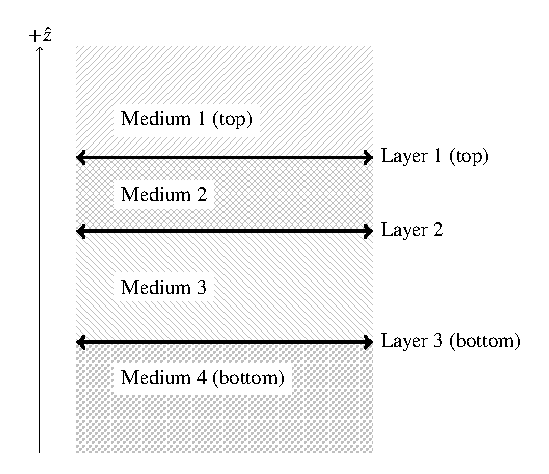
\includegraphics[width=\columnwidth]{Fig-layers/Fig-layers.pdf}
    \caption{An example diagram of a layered assembly with 3 layers
    and 4 participating media.
    \label{fig:assembly}}
\end{center}
\end{figure}

\subsection{Basics of program usage}

As \texttt{layered-sqt} is a command-line tool, it runs
on the command line, whereby it scans command-line arguments for
(optional) configuration flags and a (required) input filename
appearing somewhere as a positional argument, i.e., an argument 
not consumed by a flag. It then parses the input file, simulates 
the emergent BSDF,
and writes the results to a RAW-format file ready for conversion to
SQT-format via \texttt{raw2sqt}. For instance, 
\begin{verbatim}
$ ./layered-sqt example.lsqt -p 50000 \
  -o example.raw
\end{verbatim}
simulates a layered assembly as described in \texttt{example.lsqt} 
with 50,000 paths, and writes the emergent BSDF in plain-text RAW-format to
\texttt{example.raw}. To convert the BSDF to SQT-format, which is necessary
for use in DIRSIG, run
\begin{verbatim}
$ ./raw2sqt example.raw
\end{verbatim}
which will write a new file \texttt{example.sqt}.

Two of the most common flags appear above, namely
\texttt{-p} (or \texttt{--path-count}) to specify the number of paths used in
the simulation and \texttt{-o} (or \texttt{--output}) to specify the output 
filename. To see a list of all acceptable flags with brief descriptions and 
default values, pass \texttt{-h} (or \texttt{--help}), or simply run 
\texttt{layered-sqt} with no filename. As an aside,
\texttt{layered-sqt} verifies parameters specified in command-line flags
as well as keyword arguments specified in the input LSQT file.
In the event that something has an unreasonable value, the program
issues an error and fails in a controlled manner.

Lastly, \texttt{layered-sqt} recognizes the single dash filename 
``\texttt{-}'' as standard input. So, it is possible to pipe the 
(presumably LSQT format) output of a script into \texttt{layered-sqt} 
directly, if this happens to be convenient. As a trivial example,
\begin{verbatim}
$ cat example.lsqt | \
  ./layered-sqt -p 50000 -o example.raw -
\end{verbatim}
is equivalent to just passing \texttt{example.lsqt}.

\section{Tutorial}

This section provides a series of progressively more interesting
``learn-by-doing'' tutorials, which should naturally introduce the
concepts and features in \texttt{layered-sqt}. To get started, create
a working directory \texttt{lsqt-tutorial} and link the relevant programs
for easy access. From one of the Carlson CIS servers, 
type the following commands:
\begin{verbatim}
$ mkdir lsqt-tutorial && cd lsqt-tutorial
$ TMP_PATH=/cis/phd/mgs8033/layered-sqt/bin
$ ln -s $TMP_PATH/layered-sqt
$ ln -s $TMP_PATH/layered-sqt-lssview
$ ln -s /dirs/pkg/dirsig/bin/raw2sqt
\end{verbatim}

\subsection{Hello, world}

Let's start with something mind-numbingly simple---a 100\% 
reflective Lambertian surface. First, create and enter a 
sub-directory \texttt{tutorial1},
\begin{verbatim}
$ mkdir tutorial1 && cd tutorial1
\end{verbatim}
Using whatever text-editing program you prefer, create a 
plain-text LSQT file $\texttt{Lambertian.lsqt}$ with three lines:
\begin{lstlisting}
Medium
Layer z=0 LambertianBsdf fR=1 fT=0
Medium
\end{lstlisting}
As an aside, LSQT format input is syntax-highlighted in this 
document. However, syntax-highlighting files/add-ons are not
available (yet) for any text editor.

Now, run \texttt{layered-sqt} on \texttt{Lambertian.lsqt}, 
\begin{verbatim}
$ ../layered-sqt Lambertian.lsqt
\end{verbatim}
which should write two new files: \texttt{Lambertian.lsqt.lss} and
\texttt{Lambertian.lsqt.raw}. As stated in the introduction, we may
convert the plain-text RAW file to a binary SQT file for use with 
DIRSIG by running \texttt{raw2sqt},
\begin{verbatim}
$ ../raw2sqt Lambertian.lsqt.raw
\end{verbatim}
which generates the final SQT file \texttt{Lambertian.lsqt.sqt}
suitable for use in a DIRSIG scene.

Now, what is the LSS file?
\emph{LSS} is an initialism for \emph{LSQT-Slice}, which is the
name of the internal file format \texttt{layered-sqt} uses to store 
simulation data, and it is useful 1) for previewing the layered BSDF
\emph{without setting up and rendering a DIRSIG scene}, and 2) for
simulating a layered BSDF progressively, with multiple runs of 
\texttt{layered-sqt}.

Run \texttt{layered-sqt-lssview} to preview the Lambertian BRDF.
\begin{verbatim}
$ ../layered-sqt-lssview Lambertian.lsqt.lss
\end{verbatim}
This should write a new file, \texttt{Lambertian.lsqt.lss.png}, which 
is a 512x512 rendering of the BSDF applied to a ball. When connected 
to the CIS server with X-window support (from a Linux machine, log-in 
with \texttt{ssh -X}), this image may be viewed by running \texttt{eog}.
\begin{verbatim}
$ eog Lambertian.lsqt.lss.png
\end{verbatim}

Importantly, \texttt{layered-sqt-lssview} is \emph{not} a full-blown
path-tracer, and may not perfectly represent how the BSDF will appear
in DIRSIG. It only accounts for the direct (first bounce) contributions 
of a few directional light sources, and it further uses tone-mapping and
sRGB correction, such that the output image is not suitable for any
radiometric analysis. The intended use of this preview image is to 
determine if a simulated BSDF is suitably convergent/noise-free.

TODO

\section{Documentation}
\label{sec:doc}

This section documents the properties of participating media and 
scattering layers in more detail, and enumerates the available 
scattering models for media and layers, and how to specify them in 
LSQT format. Note that ``phase function'', ``BRDF'', and ``BSDF'' are
specific types of scattering models. In particular,
\begin{itemize}
    \item a \emph{phase function} is a scattering model which accounts
        for volume-scattering within a participating medium,
    \item a \emph{BRDF}, i.e., a \emph{Bidirectional Reflectance Distribution 
        Function}, is a scattering model which accounts for only reflection at 
        a surface, and
    \item a \emph{BSDF}, i.e., a \emph{Bidirectional Scattering Distribution 
        Function}, is a scattering model which accounts for reflection and 
        transmission at a surface.
\end{itemize}

Note that phase functions are normalized by 
definition, as volume-absorbtion is accounted for by a separate parameter. 
BRDFs and BSDFs, however, account for absorption as well as scattering, 
and so are only normalized if the model is non-absorbing (in other words,
perfectly energy conserving). To state all of this more rigorously, a
phase function $p$ is normalized with respect to integration over 
incident directions $\omega_i$, such that
\begin{equation*}
    \int_{\mathcal{S}^2} p(\omega_o\to\omega_i) \diff{\omega_i} = 1.
\end{equation*}
However, a BRDF/BSDF $f$ is only normalized as such if it is 
non-absorbing,
\begin{equation*}
    \int_{\mathcal{S}^2} f(\omega_o\to\omega_i) \diff{\omega_i} = 1
    \iff \text{$f$ is non-absorbing.}
\end{equation*}

As this ought to suggest---this document follows the convention that BRDFs 
and BSDFs contain an implicit cosine-weighting with respect to incident
direction. This is often written explicitly elsewhere in the literature,
such that the above normalization condition is written as
\begin{equation*}
    \int_{\mathcal{S}^2} f(\omega_o\to\omega_i) \verts{\cos{\theta_i}}
    \diff{\omega_i} = 1.
\end{equation*}
We effectively make the substitution $f\gets f|{\cos{\theta_i}}|$.

\subsection{Participating media}
\label{sec:doc-participating-media}

A medium is characterized by its 
absolute index of refraction $\eta \ge 1$, its absorption coefficient 
$\mu_a \ge 0 $, its scattering coefficient $\mu_s \ge 0$, and a local
phase function model.

To specify a medium, simply type the name \namett{blue}{Medium} followed
by (optional) keywords arguments \texttt{eta}, \texttt{mua}, and
\texttt{mus} for $\eta$, $\mu_a$, and $\mu_s$ respectively. Keyword 
arguments for a medium have default values \texttt{eta=1}, \texttt{mua=0}, 
\texttt{mus=0}, such that any may be omitted for brevity.
If $\mu_s > 0$, the keyword arguments must be followed by the name 
of the desired phase function, followed by any keyword arguments for the 
phase function. If $\mu_s = 0$, it is not necessary to specify a phase function
since no scattering occurs.

As the defaults may suggest, \texttt{layered-sqt} considers that vacuuum 
is just a medium with refractive index 1 which neither absorbs nor scatters. 
So,
\begin{lstlisting}
Medium
\end{lstlisting}
specifies vacuum. Note---the implementation requires that top and 
bottom media be non-absorbing and non-scattering, such that $\mu_a=\mu_s=0$,
and issues an error if this requirement is not met.

\subsubsection{Henyey-Greenstein phase}

The Henyey-Greenstein phase function is given by 
\begin{equation*}
    p(\omega_o\to\omega_i) = 
    \frac{1}{4\pi}
    \frac{1-g^2}{(1+g^2+2g\omega_o\cdot\omega_i)^{3/2}}
\end{equation*}
with shape parameter $g\in(-1,1)$. It may be helpful to note 
that $g$ is the mean cosine of the scattered direction with respect to the 
incident direction, such that $p$ becomes forward scattering as $g\to1$, 
backward scattering as $g\to-1$, and uniformly/isotropically scattering 
as $g\to0$.

To specify the Henyey-Greenstein phase in LSQT format, use the name
\namett{purple}{HenyeyGreensteinPhase} followed by the (optional) keyword 
argument \texttt{g} for $g$, which is zero by default. For example,
\begin{lstlisting}
Medium mus=1 HenyeyGreensteinPhase g=-0.22
\end{lstlisting}
specifies a moderately back-scattering medium.

\subsubsection{Rayleigh phase}
The general form of the Rayleigh phase function is given by
\begin{equation*}
    p(\omega_o\to\omega_i) = 
    \frac{3}{16\pi}
    \bracks{
        \frac{1 + 3\gamma}{1 + 2\gamma} +
        \frac{1 -  \gamma}{1 + 2\gamma} (\omega_o\cdot\omega_i)^2}
\end{equation*}
where
\begin{equation*}
    \gamma = \frac{\rho}{2 - \rho}
\end{equation*}
where, in turn, $\rho \in [-1, 1]$ is a shaping parameter known as 
the \emph{depolarization factor}. The simpler, more common form of the
Rayleigh phase function is given by
\begin{equation*}
    p(\omega_o\to\omega_i) = \frac{3}{16\pi}(1 + (\omega_o\cdot\omega_i)^2),
\end{equation*}
which is obtained by setting $\rho = 0$. 

The Rayleigh phase function prefers parallel scattering
to perpendicular scattering. That is to say, scattering in directions 
perpendicular to the direction of propagation is diminished, and scattering 
is symmetric in terms of forward- versus back-scattering. This effect is 
maximized as $\rho \to -1$ and minimized as $\rho \to +1$. Note that $p$ 
becomes uniformly/isotropically scattering in the limiting case $\rho = +1$.

To specify the Rayleigh phase function in LSQT format, use the name 
\namett{purple}{RayleighPhase} followed by the (optional) keyword argument
\texttt{rho} for $\rho$, which is zero by default. For example,
\begin{lstlisting}
Medium mus=1 RayleighPhase rho=-0.5
\end{lstlisting}
specifies a medium with an exaggerated ``Rayleigh effect'' relative to the
common form where $\rho=0$.

\subsection{Layers}
\label{sec:doc-layers}

A layer is characterized by its $z$-height and 
a local BSDF model. As different BSDF models require different 
parameters, there is a different ``type'' of layer for each 
BSDF model implemented in \texttt{layered-sqt}. 

Every layer accepts $z$-height as a parameter, so every line describing a 
layer must begin with the name \namett{blue}{Layer} followed by the (required)
keyword argument \texttt{z}. This is followed in turn by the name of the 
desired BSDF, followed by any keyword arguments for the BSDF. For example,
\begin{lstlisting}
Layer z=1 NullBsdf
\end{lstlisting}
specifies a layer at $z$-height 1 with a null BSDF. As explained in 
the next sub-section, a null BSDF is a special case which accepts no additional
keyword arguments.

The implementation requires that layers appear in top-to-bottom order,
such that the $z$-heights of subsequent layers in an LSQT file are
strictly decreasing. If this condition 
is violated, the implementation issues an error and exits.

\subsubsection{Null BSDF}

At times, it is desirable to separate participating media 
\emph{without} scattering at a layer. This is possible in
\texttt{layered-sqt} by assigning a null BSDF with name 
\namett{purple}{NullBsdf}, which may be interpreted as a 100\% 
transmissive directional delta function in the direction a 
ray is already traveling. This is useful, for example, to model a 
layer of dust on top of a surface. To do so, we might specify the 
following LSQT file
\begin{lstlisting}
Medium
Layer z=1 NullBsdf
Medium mus=1 HenyeyGreensteinPhase g=0.2
Layer z=0 LambertianBsdf fR=1 fT=0
Medium
\end{lstlisting}
which describes a layer of forward-scattering ``dust'' on top 
of a 100\% reflective Lambertian surface.

\begin{figure*}
\begin{center}
    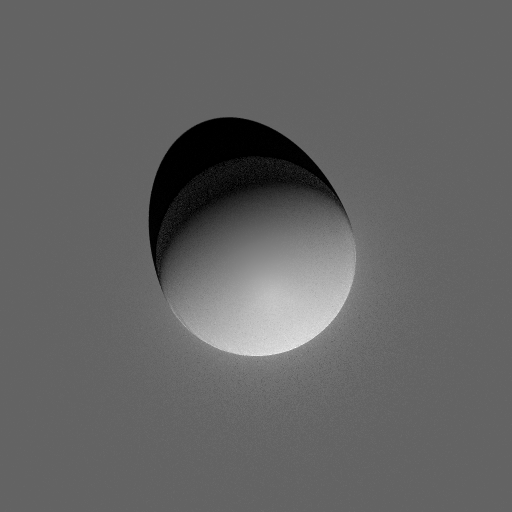
\includegraphics[width=0.4\linewidth]{example1.png}\hspace{0.05\linewidth}%
    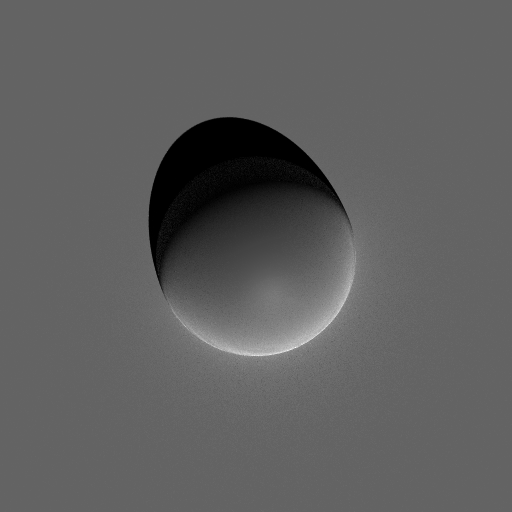
\includegraphics[width=0.4\linewidth]{example2.png}
    \caption{A sphere with an LSQT BRDF on a Lambertian ground plane 
        rendered from above with DIRSIG5. The LSQT BRDF models a
        dusty dielectric substrate---from top to bottom, we have a 
        vacuum medium, a null BSDF layer, a slightly back-scattering 
        medium with $g=-0.2$, a decently smooth microsurface dielectric 
        BSDF layer, a transparent medium with $\eta=1.5$, 
        and a Lambertian BRDF layer. On the left, the Lambertian
        layer has $f_R=0.8$. On the right, the Lambertian layer has 
        $f_R=0.4$, such that the backscattering due to ``dust'' is
        more obvious. All other parameters are the same in both images.}
\end{center}
\end{figure*}

\subsubsection{Lambertian BSDF}

The Lambertian BSDF models a uniformly scattering surface which 
may reflect, transmit, or both. That is, the (cosine-weighted)
scattering function is
\begin{equation*}
    f(\omega_o\to\omega_i) =
    \frac{|\cos{\theta_i}|}{\pi}
    \begin{cases}
        f_R & \text{$(\omega_o, \omega_i)$ in same hemisphere}\\
        f_T & \text{otherwise}
    \end{cases}
\end{equation*}
where $f_R$ and $f_T$ specify the amount of incident energy 
reflected and transmitted respectively. Both $f_R$ and $f_T$ should
be non-negative numbers such that $f_R + f_T \le 1$ for this to be
physically plausible. In the event that $f_R + f_T = 1$, this is
perfectly energy-conserving.

To specify the Lambertian BSDF in LSQT format, use the name
\namett{purple}{LambertianBsdf} followed by keyword arguments 
\texttt{fR} and \texttt{fT} for $f_R$ and $f_T$ respectively. The 
implementation requires that the values of \texttt{fR} and \texttt{fT} 
be physically plausible, i.e., non-negative numbers whose sum does not exceed 1.
For example,
\begin{lstlisting}
Layer z=2.2 LambertianBsdf fR=0.8 fT=0.1
\end{lstlisting}
specifies a Lambertian surface at $z$-height 2.2 which is 80\% reflective,
10\% transmissive, and 10\% absorptive. 

\subsubsection{Microsurface Lambertian BRDF}

A microsurface is thought 
to be an infinitesimally thin cloud of microfacets, where each facet 
is thought to scatter light according to another, simpler BSDF. The 
cloud is characterized geometrically by 1) a distribution of the
slopes of the facets and 2) a distribution of the heights of the facets,
which are assumed to uncorrelated, such that the facets are discontinuous. 
The distribution of slopes is parameterized by its so-called roughness
$\alpha$ (more generally, anisotropic roughness $\alpha_x$, $\alpha_y$).
As $\alpha\to\infty$, the distribution of slopes widens and the emergent
BSDF appears rougher. As $\alpha\to0$, the distribution of slopes collapses,
recovering the initial, simpler BSDF in the limiting case $\alpha=0$.

As given in \cite{Heitz:16},
the microsurface Lambertian BRDF is a multiple scattering (stochastic)
microfacet model wherein facets are assumed to be Lambertian reflectors. 
This is particularly useful for representing rough diffuse surfaces. The 
implementation in \texttt{layered-sqt} is parameterized by
roughness $\alpha>0$, the Lambertian BRDF coefficient 
$f_R \in [0,1]$, and the number of local stochastic process 
iterations $n_{\text{iter}} \ge 1$. For rougher microsurfaces 
(say, $\alpha > 0.4$), it is typically more efficient to increase 
$n_{\text{iter}}$ rather than the global path count.

To specify the microsurface Lambertian BRDF 
in LSQT format, use the name 
\begin{lstlisting}
MicrosurfaceLambertianBrdf
\end{lstlisting}
followed by (optional) keyword arguments 
\texttt{alpha}, \texttt{fR}, and \texttt{iter\_count} for $\alpha$,
$f_R$, and $n_{\text{iter}}$ respectively. By default, \texttt{alpha=0.5},
\texttt{fR=1}, and \texttt{iter\_count} is chosen to be 1, 2, 4, or 6 
depending on \texttt{alpha}. For reference, $\alpha < 0.1$ is very smooth, 
$0.1 < \alpha < 0.8$ is somewhat rough, and $0.8 < \alpha$ is very rough.
Furthermore, multiple scattering may be disabled by the keyword argument
\begin{lstlisting}
use_multiple_scattering=false
\end{lstlisting}
in which case only the single scattering term is computed. It is 
important to note that, if multiple-scattering interactions are 
ignored, then setting \texttt{fR=1} does not guarantee that the BRDF 
is perfectly energy conserving. 
For small roughness values (say, $\alpha < 0.1$), the energy carried by 
multiple scattering interations is insignificant, and so this may not be a
concern. For large roughness values however, multiple scattering is important
to prevent energy loss.

\subsubsection{Microsurface dielectric BSDF}

The microsurface dielectric BSDF follows the same logical construction as 
the microsurface Lambertian BRDF, except the constituent BSDF assigned to the
facets is the delta Fresnel mirror BSDF. The implementation in 
\texttt{layered-sqt} is parameterized by roughness $\alpha > 0$, a scaling
factor for the Fresnel mirror BRDF $k_R \in [0, 1]$, a scaling factor for 
the Fresnel mirror BTDF $k_T \in [0, 1]$, and the number of local stochastic 
process iterations $n_{\text{iter}} \ge 1$.

To specify the microsurface dielectric BSDF 
in LSQT format, use the name
\begin{lstlisting}
MicrosurfaceDielectricBsdf
\end{lstlisting}
followed by (optional) keyword arguments \texttt{alpha}, \texttt{kR},
\texttt{kT}, and \texttt{iter\_count} for $\alpha$, $k_R$, $k_T$, and 
$n_{\text{iter}}$ respectively. By default, \texttt{alpha=0.5},
\texttt{kR=1}, \texttt{kT=1}, and \texttt{iter\_count} is chosen to 
be 1, 2, 4, or 6 depending on \texttt{alpha}. As in the Lambertian case, 
multiple-scattering may be disabled by the keyword argument
\begin{lstlisting}
use_multiple_scattering=false
\end{lstlisting}
so that only the single-scattering term is computed. Unlike the
Lambertian case however, the single-scattering term is directly 
computable (without a stochastic process) due to the delta function 
in the Fresnel mirror BSDF---such that disabling multiple-scattering makes
\texttt{iter\_count} irrelevant. This leads to noticeably faster
simulations, though still at the cost of significant
energy loss for rough surfaces.

\subsubsection{Oren-Nayar diffuse BRDF}

TODO

{
\nocite{*}
\raggedright
\printbibliography
}
\end{document}
